\documentclass{article}
\usepackage{amsthm}
\usepackage{amssymb}
\usepackage{enumerate}
\usepackage{amsmath}
\usepackage{extarrows}
\usepackage{mathrsfs}
\usepackage[UseMSWordMultipleLineSpacing,MSWordLineSpacingMultiple=1.4]{zhlineskip}
\usepackage{lipsum}
\usepackage{pdfpages}
\usepackage[a4paper,margin=1in]{geometry}
\title{Algebra-1 Note}
\author{lin150117 }
\date{}
\newtheorem{definition}{Definition}[subsection]
\newtheorem{theorem}{Theorem}[subsection]
\newtheorem{example}{Example}
\newtheorem{remark}{Remark}
\newtheorem{corollary}{Corollary}
\newtheorem{proposition}{Proposition}
\begin{document}
\setlength{\parindent}{0pt}
\paragraph*{Exercise5.5}
\begin{proof}
    If  $ \pi  $ is an associate of an integer prime, i.e.  $ \pi=u\cdot p $,  $ p  $ is a integer prime. Then  $ \overline{\pi}=\overline{u}\cdot \overline{p}=\overline{u}\cdot p $ is associated with  $ \pi $. $ (\ast) $ \\
    If  $ \pi  $ is not an associate of an integer prime. \\Then for  $ \pi=a+bi,a,b\not=0,a,b\in \mathbb{Z} $,  $ \pi,\overline{\pi } $ are associated if and only if  $ a+bi=u\cdot(a-bi)$, where  $ u  $ is a unit, i.e.  $ u\in\{1,-1,i,-i\} $  $ \Leftrightarrow  $  $ (a+bi)=u\cdot(a-bi) $ for  $ u\in\{i,-i\} $. $ \Leftrightarrow $  $ (a,b)=(b,a) $ or $ (a,b)=(-b,-a) $.  $ \Leftrightarrow  $  $ a^2=b^2 $. \\
    Now, assume  $ a^2=b^2 $, by Theorem 12.5.2(a),  $ \pi\cdot \overline{\pi}=a^2+b^2=2a^2 $ is an integer prime or the square of an integer. $ 2|2a^2 $ $ \Rightarrow  $  $ 2a^2=2 or 4 $  $ \Rightarrow  $  $ 2a^2=2 $ ($a\in\mathbb{Z} $) So  $ \pi\cdot\overline{\pi}=2 $.\\
    If  $ \pi\cdot\overline{\pi}=2 $, i.e.  $ a^2+b^2=2 $. Since  $ \pi  $ is not an associate of an integer prime, then  $ a,b \geq 1 $,  $ \Rightarrow  $  $ a^2=b^2=1 $  $ \Rightarrow  $  $ \pi=1+i  $ or  $ \pi=1-i $  $ \Rightarrow  $  $ \pi,\overline{\pi } $ are associated.\\
    So we have proved that if  $ \pi  $ is not an associate of an integer prime, then  $ \pi  $ and  $ \overline{\pi } $ are associates if and only if  $ \pi\overline{\pi}=2 $. It implies the original problem by  $ (\ast) $ .
\end{proof}
\paragraph{Exercise5.6}
\begin{proof}
    Since  
    \begin{align}
        \mathbb{Z}[\sqrt{-3}]/(p)&\cong\mathbb{Z}[x]/(x^2+3)/(p)\\
        &\cong\mathbb{Z}[x]/(p,x^2+p)\\
        &\cong \mathbb{Z}[x]/(p)/(x^2+3)\\
        &=\mathbb{F}_p[x]/(x^2+3)
    \end{align}
     $ p  $ is prime in  $ \mathbb{Z}[\sqrt{-3}] $ $ \Leftrightarrow  $  $ \mathbb{Z}[\sqrt{-3}]/(p) $ is integral domain  $ Leftrightarrow  $  $ \mathbb{F}_p[x]/(x^2+3) $ is integral domain  $ \Leftrightarrow $  $ x^2+3 $ is prime in  $ \mathbb{F}_p[x] $ $ \Leftrightarrow $  $ x^2+3 $ is irreducible in  $ \mathbb{F}_p[x] $ since  $ \mathbb{F}_p[x] $ is PID.
\end{proof}
\paragraph{3.}Let  $ R:=\{\sum\limits_{i=0}^n a_it^i\in \mathbb{C}[t]: a_1=0\} $, which is a subring in  $ \mathbb{C}[t] $ \\
For  $ f(t)=\sum\limits_{i=0}^n a_it^i\in R, a_1=0 $, we have 
\[\varphi(a_0+\sum\limits_{3 \leq i \leq n,2|i}a_ix^{\frac{i }{2}}+\sum\limits_{3 \leq i \leq n,2|(i-1)}a_ix^{\frac{i-3 }{2}}y)=f(t)\]
Moreover, for  $ x^ay^b\in \mathbb{C}[x,y] $, we have  $ \varphi (x^ay^b)=t^{2a+3b} $ of degree  $  \geq 2 $ if  $ x^ay^b  $ is not a constant. So  $ \varphi(f) \in R $.\\
Therefore,  $ \varphi  $ can induce  $ \hat{\varphi}:\mathbb{C}[x,y]/\ker \varphi\rightarrow R $ bijection, moreover, an isomorphism since  $ R  $ is a subring in  $ \mathbb{C}[t] $.\\
So it suffices to prove the induced map  $ \mathrm{Spec}(\mathbb{C}[t])\rightarrow \mathrm{Spec}(R), p\mapsto p\cap R $ is bijective.\\
Since  $ \mathbb{C}[t] $ is PID, prime ideal in  $ \mathbb{C}[t] $ are exactly  $ (p) $, where  $ p=x+c,c\in \mathbb{C} $ prime element in  $ \mathbb{C}[t] $.\\
Then for  $ (x+c_1),(x+c_2) $ prime ideal in  $ \mathbb{C}[t] $, $ c_1\not=c_2 $ ,  $ x^3+c_1x^2\in (x+c_1)\cap R $. But if $ x^3+c_1x^2\in (x+c_2) $, then  $ x^2\in(x+c_2) $ since $ x+c_1\not\in(x+c_2) $. So  $ c_2=0 $. But now  $ x^2\not\in (x+c_1) $ $ \Rightarrow (x+c_1)\cap R\not=(x+c_2)\cap R $. Otherwise, if  $ x^3+c_1x^2\not\in (x+c_2) $, then   $ (x+c_1)\cap R\not=(x+c_2)\cap R  $. Therefore, the induced map should be injective.\\
Define  $ \mathbb{C}[t^n]=\{\sum\limits_{i=0}^n a_i t^{in}:a_i\in \mathbb{C}\} $ be a subring of  $ R $ if  $ n \geq 2 $, moreover, a PID since it is equivalent to replace  $ t  $ with  $ t^n  $ in  $ \mathbb{C}[t] $. \\
For  $ P  $ prime ideal in  $ R $. For  $ n \geq 2 $, the inclusion homomorphism  $ \mathbb{C}[t^n] \rightarrow R $  induce the map  $ \mathrm{Spec}R\rightarrow \mathrm{Spec}\mathbb{C}[t^n]$. Then  $ P\cap \mathbb{C}[t^n]  $ is a prime ideal in  $ \mathbb{C}[t^n] $. So  $ P\cap \mathbb{C}[t^2]=(t^2+c)\mathbb{C}[t^2],P\cap \mathbb{C}[t^3]=(t^3+c')\mathbb{C}[t^3] $. Let  $ c=-k^2 $ for some  $ k\in \mathbb{C} $. Since  $ (t^3+k^3)(t^3-k^3)=t^6-k^6\in (t^2-k^2)\mathbb{C}[t^2]\subset P $, $ \Rightarrow  $  $ t^3+k^3\in p$ or $ t^3-k^3\in P $. Then we have  $ t^3+k^3\in P\cap\mathbb{C}[t^3]=(t^3+c')\mathbb{C}[t^3] $ or  $ t^3-k^3\in P\cap\mathbb{C}[t^3]=(t^3+c')\mathbb{C}[t^3] $, which means  $ P\cap \mathbb{C}[t^3]=(t^3+k^3)\mathbb{C}[t^3] $ or  $ (t^3-k^3)\mathbb{C}[t^3] $.\\
WLOG, we assume that  $ P\cap \mathbb{C}[t^3]=(t^3+k^3)\mathbb{C}[t^3] $(otherewise we replace k with -k). For  $ f=\sum\limits_{i=0}^n a_it^i\in R $,  $ f=g(t^2-k^2)+rt+s $ where  $ g\in \mathbb{C}[t],r,s\in \mathbb{C}[t] $. Let  $ g=g'+mt,g'\in R $. Then  \[f=g'(t^2-k^2)+mt^3-mk^2t+rt+s \] $ g'(t^2-k^2)\in P $. Since  $ f\in R $,  $ (r-mk^2)t=0 $. So  $ f\in P  $ if and only if  $ mt^3+s\in P $ $ \Leftrightarrow $  $ mt^3+s\in (t^3+k^3)\mathbb{C}[t^3] $ $ \Leftrightarrow $ $ s=mk^3 $ $ \Leftrightarrow $  $ f(-k)=g'(-k)((-k)^2-k^2)+m(-k)^3+s=0 $ $ \Leftrightarrow  $ $ (x+k)|f $. So  $ P=(x+k)\cap R $ \\
Therefore every prime ideal  $ P  $ in  $ R  $ should be the intersection of prime ideal in  $ \mathbb{C}[t] $ and  $ R  $. Which means the induced map is surjective.\\
So the induced map  is bijective.                     
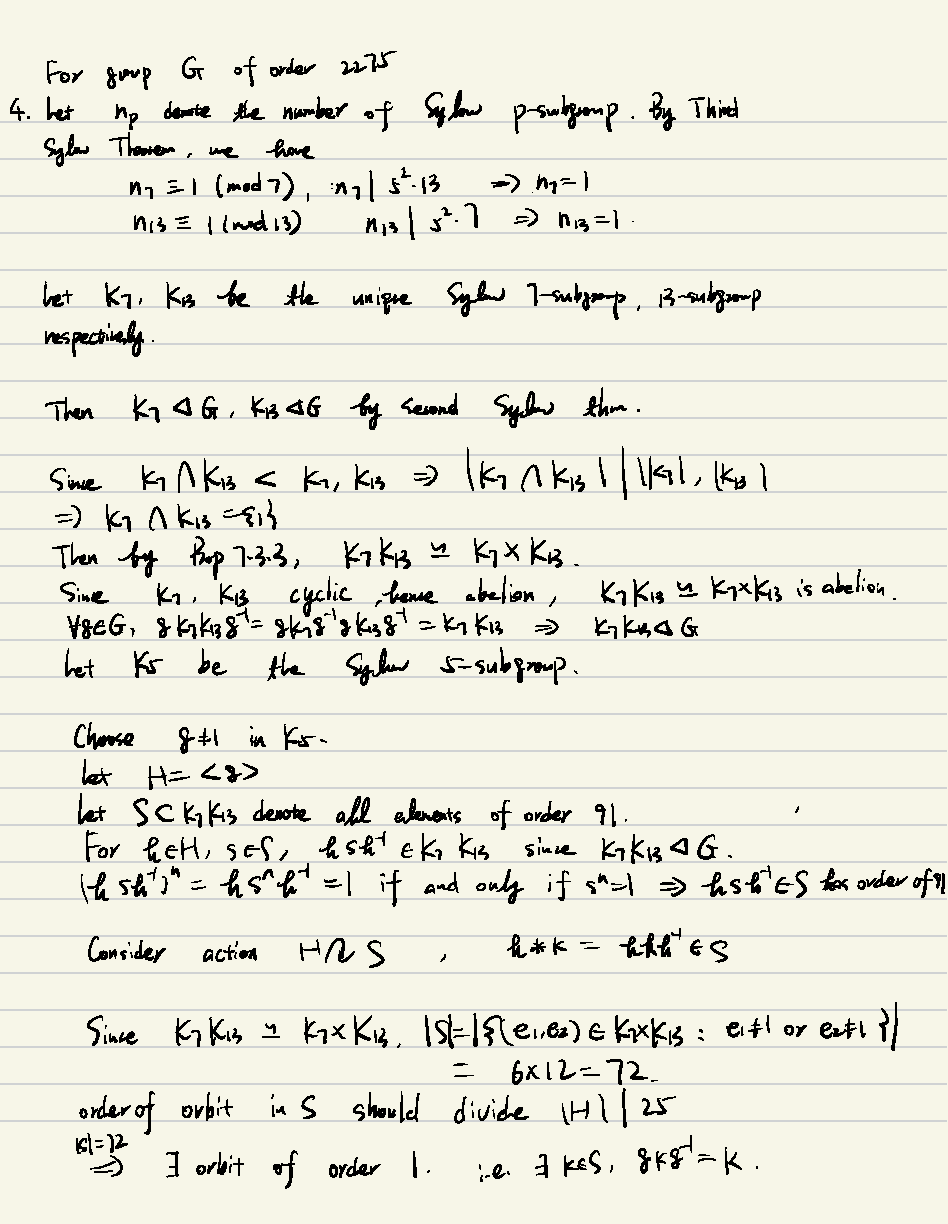
\includepdf[pages={1,2}]{代数hw.pdf}
\end{document}
